%!TEX root = thesis.tex

%
%==========================================================================================
%
\chapter{Accumulating Behavior Evaluations Over Time}
\label{chap:accumulation}

Anomalous and suspicious behavior detection becomes more challenging when agents are observed over a longer period of time. In many domains, no single event is sufficient to determine deviant behavior. Instead, multiple evaluations must be combined. This contrasts with previous chapters, which focused on the detection of a single, clearly suspicious event. 

This chapter proposes a two-step detection system, which first detects trigger events in behavior trace, and then combines the evidence to provide a degree of suspicion. The chapter specifies conditions that any reasonable detector should satisfy, analyzes  three detectors, and proposes a novel detector that generalizes a utility-based plan recognition with arbitrary utility functions.
%The results on a simulated airport domain and a dangerous-driver domain show that our new algorithm outperforms other approaches in several settings.



%\section{Definitions and Assumptions}
%\label{sec:definitions}
%\noindent



% %\subsection{Trigger Events}
% %\label{sec:events}
% %\noindent
% Trigger events can be any kind of partial observations we are able to extract from the domain. In the airport domain, one can focus on people exhibiting indications of suspicious behavior, such as taking photos of critical infrastructure, revisiting the same location, evading the area when noticed, standing in customer service but not requesting the service, etc. 
% %We focus on a rather novel descriptor we were unable to find in the literature on suspicious behavior detection at the airport. 
% We focus on a well-known detector obtained from conversations with domain experts. %and commonly used by behavior detections officers\footnote{An approach for monitoring behavior of passengers over longer periods of time relies upon security personnel such as behavior detection officers (BDOs) that patrol airport to identify passengers who display \emph{involuntary physical and physiological actions}. US Transportation Security Administration (www.tsa.gov) trained and deployed BDO officers at 161 US airports.}.
% We observe the interactions between agents at the airport, more precisely, we are interested in how a passenger behaves in the presence of a uniformed authority figure. A person exposed to a high level of stress produces behavior that indicates fear, anxiety, pressure, tension, deception, etc. Hence, it is rational for the suspicious agent to minimize contacts with the authorities. Note, that no single avoidance is enough to raise a flag, but many such events put together cause the person to be treated as suspicious. 

% %This results in a set of partial observations describing interactive behavior of a passenger. The recognition process first extracts all interactions between passengers and authority figures inside a given radius, producing a set of trajectory pairs that are transformed to relative presentation. 

% A trigger-event detection able to identify interactive behavior may rely on coupled hidden Markov models (CHMMs), which are briefly described below. The reader is referred to~\cite{Brand} for details; the CHMMs are not the main contribution of the paper.
% %To differentiate between authority-regular and authority-suspicious interactions we present an approach based on coupled hidden Markov models (CHMM). 
% %
% The observations consist of two action traces, namely the action trace of the agent of interest and the action trace of an authority agent when they are within some predefined radius. The CHMMs are able to model the complex, interactive behavior by two HMM chains, where the hidden states from one chain directly impact on the hidden states from the other chain. Figure~\ref{fig:CHMMs} illustrates the CHMM for a pair of action traces with length $l=3$. The current state $Q_t^A$ of agent $A$ is affected by both its previous state $Q_{t-1}^A$ and previous state $Q_{t-1}^B$ of the agent $B$ (similarly $Q_t^B$ is affected by $Q_{t-1}^B$ and $Q_{t-1}^A$). Each state $Q_i$ also impacts the corresponding observation state $Y_t$. For example, if the authority agent moves toward the suspicious agent, the next state of the latter takes this into account and produces an action for an avoidance maneuver. 
% %The joint distribution for a pair of traces of length $k$ can be obtained by unrolling the network until we have $k$ slices, and them multiplying together all of the conditional probability distributions. 


% \begin{figure}[!ht]
% \centering
% \includegraphics[bb=0 0 595 830, angle=-90, width=0.5\linewidth]{graphs/chmm.pdf}
% \caption{An example of CHMM for a pair of action traces with length $l=3$.}
% \label{fig:CHMMs}
% \end{figure}

% A regular passenger may not turn or do anything different in the presence of authorities, while a suspicious person will (although as described below, an observer may not have perfect observability). Therefore, we create and train two CHMMs: $\hat{N}_I$ models the interactions produced by authorities and regular passengers, while $\hat{S}_I$ models the interactions produced by authorities and suspicious passengers. For a new event (interaction) $x$ we compute the posterior probability that the event is generated with both models yielding $\hat{n}_I(x)=\Prob\{x|\hat{N}\}$ and $\hat{s}_I(x)=\Prob\{x|\hat{S}\}$, respectively. %We also experimented with more complex CHMM structures including other features such as relative speed and distance, but the results were comparable or even worse.


%As a trigger event we also extract all turns in absence of authority when the trajectory curvature exceeds a threshold value. Probabilities that a turn event was generated by suspicious $\hat{n}_T(x)$ or regular passenger $\hat{s}_T(x)$ is acquired with frequentist estimator from the learning set $D_l$.
%
%
%The second architecture (Figure~\ref{fig:CHMM-3}) incorporates additional information in the form of a model of relative speed between two agents. This model directly impacts the states of both agents. The idea behind this architecture is to improve recognition results with an additional information.
%
%Note that for an interaction of length $T$ the architectures presented in Figure~\ref{fig:CHMMs} are unrolled to $T$ slices. %(similar as in Figure~\ref{fig:HMM-4}). 


%\begin{figure}[!ht]
%\centering
%\subfigure[]{
%\includegraphics[width=0.25\linewidth]{CHMM-2}
%\label{fig:CHMM-2}
%}
%\subfigure[]{
%\includegraphics[width=0.25\linewidth]{CHMM-3}
%\label{fig:CHMM-3}
%}
%\caption{CHMM presented as 2-sliced DBN: (a) modeling actions of two agents and (b) modeling both actions and relative speed.}
%\label{fig:CHMMs}
%\end{figure}




%%%%%%%%%%%%%%%%%%%%%%%%%%%%%%%%%%%%%%%%%%%%%%%%%%%%%%%%%%%%%%%%%%%%%%%%%%%%%%%%%%%%%%%%%%%


\section{Problem Statement}
\label{sec:problem}

We target a large class of applications where no single event is sufficient to make a decision about whether or not behavior is suspicious. Instead, we face a sparse set of \emph{trigger events} that identifies interesting parts characterizing the behavior trace. 

\begin{definition}
\index{event!trigger event}
	\emph{Trigger event} $e_t$ is an evaluation of a subsequence in behavior trace $\mathbf{b}$. 
	%(s.t.\  $1 \leq i < j \leq k$)
	It is described by probabilities that the corresponding subsequence is suspicious $s(e)$ and normal $n(e)$.
\end{definition}
\noindent

Instead of constructing a behavior pattern from the complete behavior trace, only interesting subsequences are extracted and denoted as trigger events. Each event is then further analyzed as a behavior pattern and evaluated as described in the previous chapter. Multiple trigger events are combined into an event trace.

\begin{definition}
\index{event!event trace}
	\emph{Event trace} $\evec{k}$ is a totally-ordered sequence of $k$ trigger events $\evec{k}=\{e_1,e_2,...,e_k\}$.
\end{definition}

Examples include a potentially suspicious passenger who appears to turn away in the presence of security personnel, but not blatantly so; hence, no single event is enough to raise suspicion.
The main question we address is how to combine multiple events to decide whether an event trace corresponds to the normal or a suspicious agent behavior. 

%There are four challenges that need to be addressed. 
%First, there is no one significant event or incident that would help us to reach a decision immediately; a series of trigger events allows us to reach a decision. Second, we have no knowledge about the exact plans devised by a suspicious person. Third, trigger events include multiple agent interactions complicating recognition in the presence of noise. Fourth, an event's suspicion degree depends on the agent's past behavior. For example, the third suspicious event is evaluated differently than the first, since the agent's previous behavior indicates a tendency to behave suspiciously. Hence, the simple counting of suspicious trigger events cannot be applied, since it accumulates all the events linearly. Furthermore, most plan-recognition methods, which rely on a plan library, are insufficient, since plans are not known in advance.

We address the suspicious behavior detection problem in two steps, as shown in Figure~\ref{fig:two-step-detection}. The first step analyzes an action trace and the surrounding environment to detect trigger events that characterize its interesting parts. The event trace is then evaluated in second step. If the evaluation exceeds a threshold value or is large relative to other evaluations, the event is considered suspicious.


\begin{figure}[!ht]
\centering
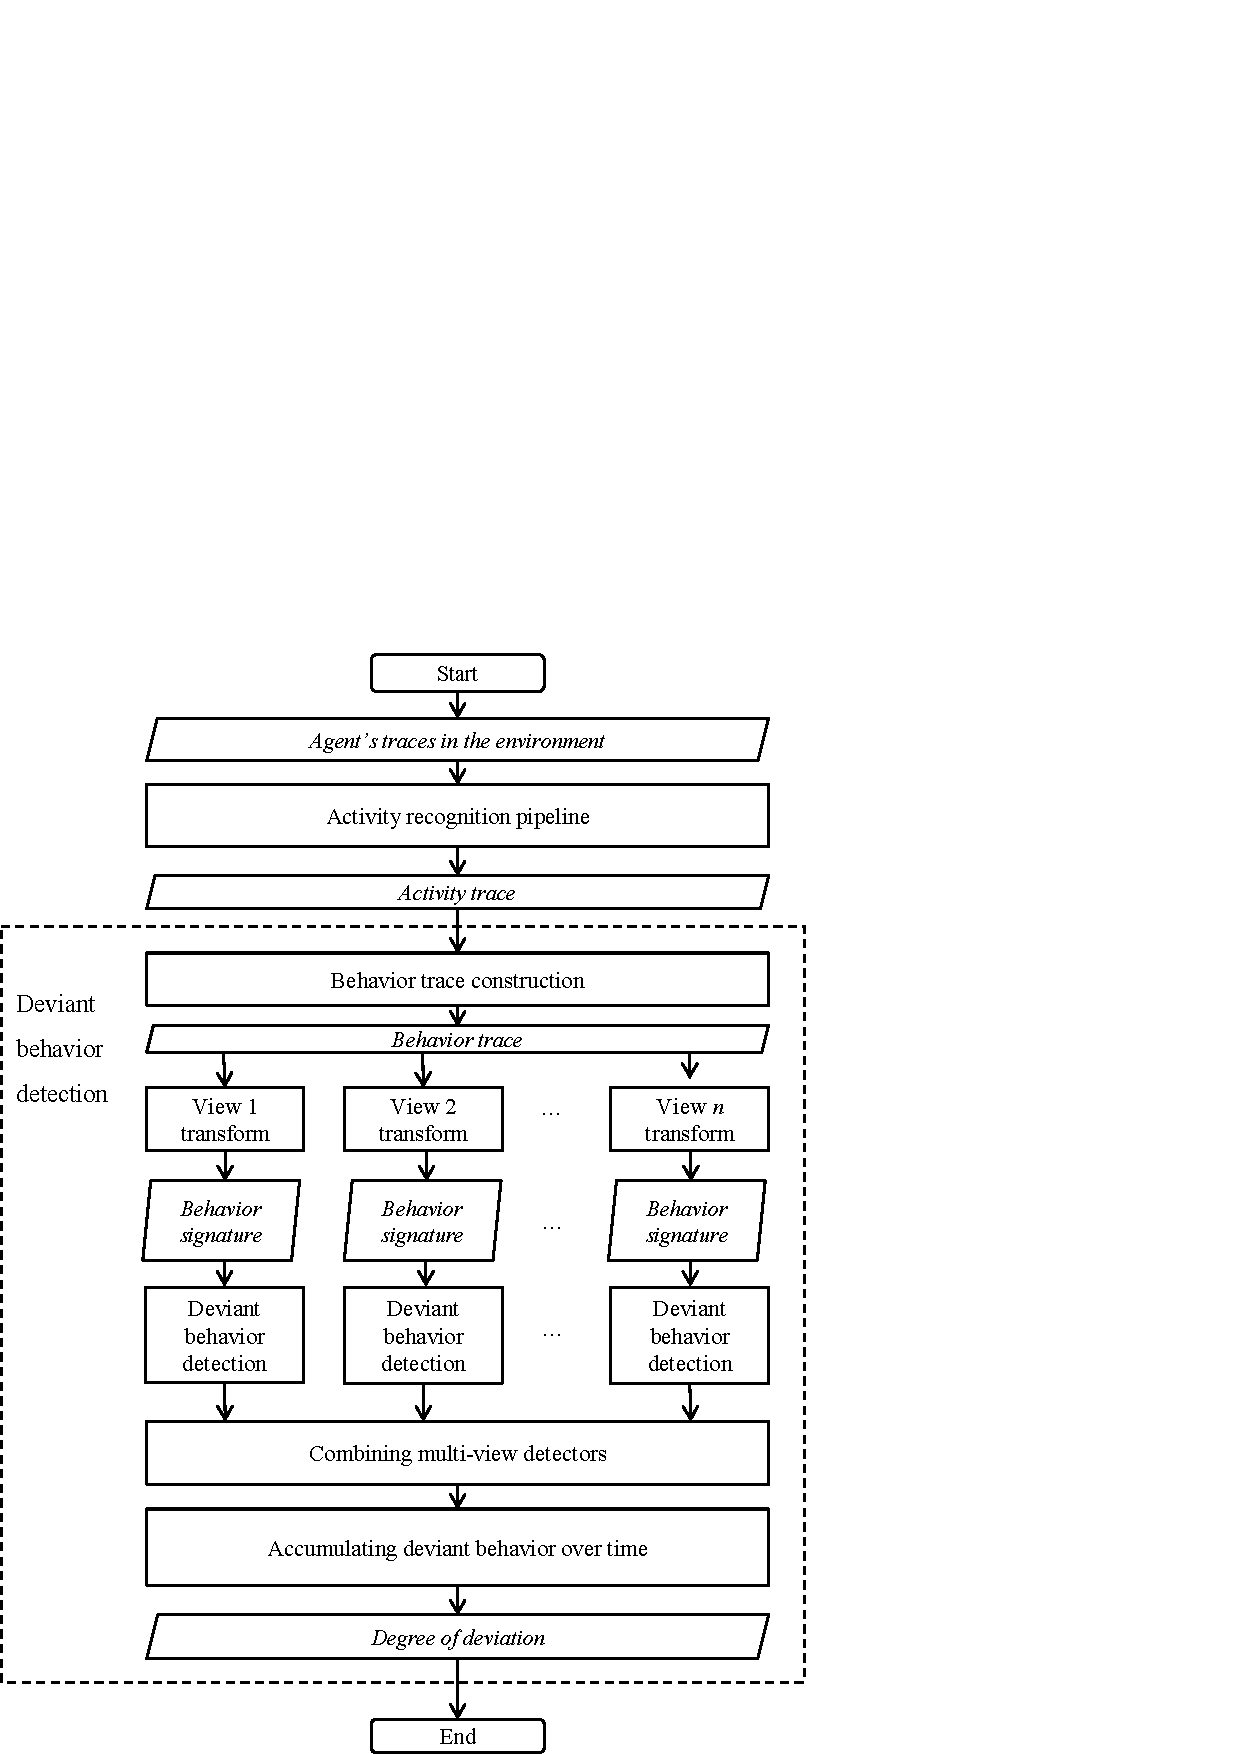
\includegraphics[width=0.6\linewidth, bb=34 10 523 530]{graphs/flowchart.pdf}
\caption{Two-step detection of suspicious behavior: (i) detection of trigger events; and (ii) detection of suspicious behavior.}
\label{fig:two-step-detection}
\end{figure}


%This paper presents a two-step approach to suspicious behavior detection from a sequence of an agent's actions. The first step detects trigger events; that is, interesting parts of the sequence that serve as evidence, and estimates the probability that an event is suspicious. For this task we present an approach using coupled hidden Markov models~\cite{Brand} that are able to model interactive behavior. The second step combines evidence from multiple events in order to determine suspiciousness.

The key contributions of this chapter are in the second step, which is defined as a decision problem: {is the behavior of an agent suspicious given a sequence of trigger events?} First, we formally describe the detection problem and specify the conditions that any reasonable detector should satisfy. Second, we analyze three detectors, namely the na{\"i}ve Bayes detector, the hidden Markov models and the utility-based plan recognition (UPR). These detectors, however, either simplify the problem or evaluate the events linearly. Finally, we present a novel detector that generalizes UPR as Function-UPR (F-UPR): we define utilities as a set of functions over state transitions and observations, and introduce an observation utility function that is especially suitable for suspicious behavior detection, since it is able to evaluate events non-linearly.
%
%The experimental evaluation on a simulated airport domain first compares the three detectors with our proposed approach. The best two approaches are additionally compared on the dangerous-driver domain.




%Our methods are general, but for illustrative purposes we will make use of the airport domain to provide examples. We treat subjects as agents in a multi-agent environment. At this point we assume that we can perfectly observe their actions. 

\section{Detection Scheme}

This section formally analyzes how to evaluate a sequence of trigger events. 
Our methods are general, but we will make use of the airport domain (Chapter~\ref{chap:lax}) to provide examples, where the goal is to detect a suspicious passenger from a surveillance camera network. Even though we will be focused on suspicious behavior detection, the same conclusion can be drawn for anomalous behavior detection. 
%We treat subjects as agents in a multi-agent environment. At this point we assume that we can perfectly observe their actions.  

We leverage the Bayesian intrusion-detection framework \citep{Helman1993} to define the problem. At each time step $t$, we observe an event $e_t$, generated by a hidden stochastic process $H$. Now suppose that $H$ is a mixture of two auxiliary stochastic processes, namely the normal process $N$ and the suspicious process $S$. The random variable $y_t=0$ if $e_t$ is generated by $N$ and $y_t=1$ if $e_t$ is generated by $S$. Since a suspicious passenger always emits a suspicious event (and a normal person a normal event), $y$ for a specific agent does not change over time. In reality, there can be many subprocesses contributing to both $N$ and $S$; that is, many normal persons with different behavior patterns. However, here we assume only a single $N$ and a single $S$ that capture all the variability. 

To this point, we assumed that an observer is able to perfectly observe whether an event is generated by $S$ or $N$. In practice, however, it may appear that a normal person emits suspicious events (or vice-versa). An observer might be limited for various reasons, such as an inability to detect characterizing features and noisy trigger-event detectors. Therefore, we relax this assumption as follows. An event $e_t$ is observed as generated by $N$ with the probability 
\begin{equation}
	n(e_t) = \Prob\{H(t)=e_t|y_t=0\}
\end{equation}
and as generated by $S$ with the probability 
\begin{equation}
	s(e_t) = \Prob\{H(t)=e_t|y_t=1\}= 1 - n(e_t).
\end{equation}
The mixture distribution of an event $e_t$ and a prior probability $\lambda$ is
\begin{equation}
  \Prob\{H(t)=e_t\} = \lambda s(e_t) + (1-\lambda) n(e_t).
\end{equation}
  

The objective of suspicious behavior detection is to identify those traces $\evec{k}=(e_1,e_2,...,e_k)$ that are likely to be suspicious activities; that is, traces $\mathbf{x}$ for which
\begin{equation}
		%\Prob\{y_t=1|H(t)=e_t, t=1,...,k\} > \tau,
		\Prob\{y=1|H(t)=e_t, t=1,...,k\} > \tau,
\label{eq:detect-sequence}
\end{equation}
is above some threshold $\tau$ or is large relative to the probability for other traces.
%
%An event $e_t$ may depend on the current step $t$ as well as on the pattern of events generated at time steps prior $t$. 
%This allows that $H$ is non-stationary, where its distribution depends both on actual time step $t$ and previously observed events, for example, if the observer identifies three out of four events in an event trace as generated by $N$, a new event will be most likely again observed as generated by $N$. 
%The non-stationary nature might reflect that: (i) agent behavior depends on his/her prior actions; (ii) agent's executing goals change over time; (iii) behavior changes over time (different population of agents); and (iv) the environment changes over time.

The reason this problem is difficult is the non-linear effect. Consider the following example: suppose we observe a person do a U-turn in front of a police officer, so such that the likelihood that this was a suspicious person becomes high. Later, we see the same person doing a half-turn in front of a police officer. This trigger event, if seen on its own, would not contribute much to the overall suspicion. However, following the initial observed turn, this new turn is a much stronger evidence to be attributed to the overall suspicion, because we bias the new event with our previous observation.

Theoretically, it might be possible to optimally detect suspicious behavior using Equation~(\ref{eq:detect-sequence}). Unfortunately, this is usually not the case in practice. 
%
%TODO: why is this difficult? Why not use existing methods?
%
To see this, let us assume a prior probability $\lambda=\Prob\{y_t=1, t=1, ..., k\}$. In most cases, $\lambda$ is close to $0$, since in real-world applications suspicious activities are rare. 
%
Let the stochastic processes $N$, $S$ and $H$ denote $n(\evec{k})=\Prob\{H(t)=e_t, t=1, ..., k|y=0\}$, ~~$s(\evec{k})=\Prob\{H(t)=e_t, t=1, ..., k|y=1\}$, ~and~~ $h(\evec{k}) = \Prob\{H(t)=e_t, t=1, ..., k\}$, respectively.
Using Bayes theorem we can derive from Equation~(\ref{eq:detect-sequence})
\begin{eqnarray}
\label{eq:bayes}
        \lefteqn {\Prob\{y=1|H(t)=e_t, t=1,...,k\} = \frac{\lambda \cdot s(\evec{k})}{h(\evec{k})} = } \\
		%&&=\frac{\Prob\{y_t=1, t=1, ..., k\} \cdot \Prob\{H(t)=e_t|y_t=1, t=1,...,k\}}{\Prob\{H(t)=e_t|t=1,...,k\}} \nonumber\\
		%&&=\frac{\lambda \cdot s(\evec{k})}{h(\evec{k})} =\nonumber\\
		&&=\frac{\lambda \cdot \prod_{t=1}^k s(e_t|e_i, _{i=t-1,...,1})}{\lambda \prod_{t=1}^k  s(e_t|e_i, _{i=t-1,...,1}) + (1-\lambda) \prod_{t=1}^k  n(e_t|e_i, _{i=t-1,...,1})}. \nonumber
\end{eqnarray}

To this point, we implicitly assumed that the distributions $\lambda$, $n$, and $s$ are reliably estimatable. The degree to which this assumption is valid depends on our detection capability.
%
%For each trace $tr_j=\{e_1,...,e_n\}, tr_j \in D_l$ we have a corresponding trace $Y_j=\{y_1, ..., y_n\}$ that specifies whether events were generated by normal or suspicious agent, meaning $y_1=y_2=...=y_n$. 
Suppose we have a sufficiently large dataset $\mathcal{D}_l$ of labeled event traces: we can estimate the prior probability $\lambda$  using the relative frequency, presenting the number of traces generated by a suspicious agent divided by the total number of traces (since traces can be of different lengths, the quotient is normalized by the traces' length).
%
%TODO: estimation of $\lambda$, $n()$ and $s()$. Prior probability $\lambda$ can be estimated 
%
Note that in order to compute $\Prob\{H(t)=e_t, t=1,...,k|y=1\}$ we have to evaluate
\begin{eqnarray}
\label{eq:bayes-opt}
	&s(e_1) \cdot s(e_{2}|e_1) \cdot ... \cdot s(e_k|e_{k-1},...,e_1).
\end{eqnarray}
%which presents a a challenge since we need to specify (or estimate) conditional probabilities of an event for all possible combinations of history. 
While some first terms, that is, $s(e_t), s(e_t|e_{t-1})$, can still be estimated, latter term estimation, including increasingly more history, becomes less and less reliable. In real-world applications, we have no direct knowledge of the conditional probabilities values; that is, we are unable to specify the probability of an event given all the possible combinations of history. For this reason, we must approximate the Bayes optimality in general. In particular, we will be concerned with estimating $\Prob\{y=1|H(t)=e_t, t=1,...,k\}$ using approximate approaches.

%Problems ??:\\
% - it is hard to get probabilities for every possible history length\\
% - we need to simplify: limited history (we may lose important information), event independence (but events are not independent)\\
% - also: does not incorporate observer's bias (solution: UPR)\\
% - solution: heuristics -- scoring functions




%\subsection{Well-behaved Scoring Functions}
%\noindent
Given an event trace, some events may appear suspicious and some not. Hence, detection systems must have a scoring function that combines the evidence. Function output is interpreted as the degree of suspicion attributed to the event trace. Although any two scoring functions need not be exactly the same, we can specify the conditions that any reasonable scoring function must satisfy.  The class defined below appears to be both natural and general.

The detection system can employ a \emph{scoring function} $f$ that interprets events to produce a score characterizing the overall suspicion of the trace. Given a threshold value $\tau$ and an event trace $\evec{k}$, we can classify $\evec{k}$ as suspicious if $f(\evec{k}) \geq \tau$.
\begin{definition}
	A scoring function $f$ over a trace of events $\evec{k}$ is a function
	$$
	f: \bigcup_{k=1}^{K} \evec{k} \rightarrow  \mathbb{R}.
	$$
%	$$
%	f: <\{s(e_1), n(e_1), ..., s(e_n), n(e_n)\}>^{2n} \rightarrow  R
%	$$
\end{definition}
The function $f$ assigns a real value to any trace $\evec{k}$ of length $k=1,...,K$. 

\noindent
Let $\Delta(e_t)$ decide whether a single event $e_t$ is suspicious or not given a threshold $\tau'$:
\begin{eqnarray}
\label{eq:delta}
        \Delta(e_t) = 
			\begin{cases}
		   1; & \text{if } {s'}(e_t) \geq {\tau'} \\
		   0; & \text{else }
		  \end{cases},\\
		{s'}(e_t)=\frac{\lambda \cdot {s}(e_t)}{\lambda \cdot {s}(e_t) + (1-\lambda) \cdot {n}(e_t)}.
\end{eqnarray}

\begin{definition}
A class of \emph{well-behaved} functions consist of scoring functions s.t. $\forall \evec{k}, e_{k+1}:$
\begin{eqnarray*}
f( \evec{k}, e_{k+1} ) \geq f(\evec{k}) &&\textrm{ if } \Delta(e_{k+1}) = 1, \\
f( \evec{k}, e_{k+1} ) \leq f(\evec{k}) &&\textrm{ if } \Delta(e_{k+1}) = 0.
\end{eqnarray*}
\end{definition}
\noindent The conditions imply that the scoring function $f$'s evaluation increases when a new suspicious event is added to the trace, and decreases when a normal event is added to the trace. The well-behaved scoring functions are motivated by the key observation that a suspicious event $e_{k+1}$ (that is, $\Delta(e_{k+1})=1$) is more likely to be generated by a suspicious process $S$ than a normal process $N$, regardless of the history $\evec{k}$, that is, 
\begin{eqnarray*}
s(e_{k+1}|\evec{k}) \geq n(e_{k+1}|\evec{k}) &&\textrm{ if } \Delta(e_{k+1})=1 \textrm{ and }\\
s(e_{k+1}|\evec{k}) \leq n(e_{k+1}|\evec{k}) &&\textrm{ if } \Delta(e_{k+1})=0.
\end{eqnarray*}
%Given such assumptions the likelihood that a trace is emitted by a suspicious process as given by Equation (\ref{eq:bayes}) is a well-behaved function. 

\section{Detectors}
\label{sec:acc-detectors}
\index{detector}
%Several approaches have been proposed to tackle the problem of suspicious behavior detection and the literature is vast. Much of it is only superficially related, in the sense that the overall goals may be the same, but the application domains and the applied methods differ. For instance, detecting suspicious behavior from video surveillance cameras pursue the same goal, but the focus is on video analytics \cite{Visontai}. Similarly, we will not address here related work on suspicious behavior detection from video features, for example, \cite{Arsic,Bak2009,Barbara2008} or anomalous trajectory shapes \cite{Nguyen2005,Piciarelli,Sillito2008,Tung2010}. We focus instead on the observable actions of agents that reveal their intentions. We thus limit ourselves to related research within recognition of multiple events giving a special focus to Hidden Markov Models (HMMs)~\cite{Rabiner1989} and Utility-based Plan Recognition (UPR)~\cite{Avrahami-zilberbrand2007}. 
%Geib and Goldman~\cite{Geib2002}, for example, addressed the problem of recognizing the plan abandonment resulting in an explosion of hypothesis, which was solved by probabilistic plan revision. However, the main difference between related work in plan recognition and our approach is that we do not assume any plan library but rather evaluate events.


%TODO: optimal detection is not possible...

%Given any set of rules, a new transaction may pass some rules and fail others. 
\noindent
This section analyzes approaches that determine whether an event trace is suspicious. First, we discuss the na{\"i}ve Bayes detector that relaxes the initial assumptions. Next, we discuss an approach that directly tackles estimating the likelihood that a trace was generated by a suspicious process using HMMs. Finally, we analyze an approach based on plan recognition and present two extensions: (i) we define utilities as a potential function; and (ii) we present an observation utility function able to address non-linear accumulation.

%They estimate conditional probabilities either by simplifying the assumptions or by modeling the conditional probabilities with another process. Finally, as an alternative, we discuss approaches that do not explicitly estimate the probability. Instead, they use heuristics, statistical measures, and plan recognition framework to provide an evaluation that the trace is generated by suspicious agent.

%There are two approaches to detecting deviant behavior~\cite{Avrahami-Zilberbrand2009}: \emph{suspicious} and \emph{anomalous} behavior detection. The first approach assumes a behavior library that encodes \emph{negative behavior}, and thus recognizing observed behavior corresponds to identifying a match in the library. The second approach uses the behavior library in an inverse fashion, meaning that the library encodes only \emph{positive behavior}. When an observed behavior cannot be matched against the library it is considered as anomalous. 




\subsection{Na{\"i}ve Bayes Detector}
%myopic approximation of Bayesian
%The resulting Bellman equations are identical to the above equations for Bayesian planning, except the belief state is not updated on the right-hand side
\noindent
A naive approach assumes that events are independent, 
%(i) events are independent and (ii) processes $\hat{N}$ and $\hat{S}$ are stationary, 
which means that the current event depends only on the current time step $t$ and not on the time steps prior to $t$. The evaluation of Equation~(\ref{eq:bayes}) is simplified using the naive assumption:
\begin{eqnarray}
\label{eq:naive-bayes}
    \lefteqn {\Prob\{y=1|H(t)=e_t, t=1,...,k\} = }\nonumber \\
	&&\frac{\lambda \cdot \prod_{t=1}^{k}\hat{s}(e_t)}{\lambda \cdot \prod_{i=1}^{k}\hat{s}(e_t) + (1-\lambda) \cdot \prod_{i=1}^{k}\hat{n}(e_t)}. 
\end{eqnarray}
We have to evaluate the probability $\Prob\{H(t)=e_t|y_t\}$ that an event is generated by both a normal process $\hat{n}(e_t)$ and a suspicious process $\hat{s}(e_t)$, which is tractable in terms of evaluation. The approaches for estimating $\hat{n}$ and $\hat{s}$ may include a frequentist estimator, hidden Markov models, k-nearest neighbors, neural networks, etc. We showed an approach using CHMM in Section~\ref{sec:ar:interactions}. An evaluation of the event trace is also well behaved when $\tau'=\lambda$.

In practice, the model may be oversimplified by the assumptions; however, we will use it as a baseline in our experiments.


\subsection{Hidden Markov Models}
\noindent
\index{hidden Markov models}
A conditional probabilities estimation including the history can be encoded with HMMs \citep{Rabiner1989}, as described in Section~\ref{sec:ar:hmm}. 
%A HMM is a temporal probabilistic model with two embedded stochastic processes: an unobservable (hidden) process $Q$, which can be observed only through another (visible) stochastic process $O$. Each state in $Q$ has state-transition probabilities (which are visible) and a probability distribution over the possible values of $O$. The key assumption is that the current hidden state of the agent is affected only by its previous state. 
%
Now suppose we create an HMM to estimate $\Prob\{H(t)=e_t|y=1, t=1,...,k\}$; more precisely, it models the probability that an event trace is generated by a suspicious agent. The hidden states of the process $Q$ may be referred to as internal states presenting the suspicious agent's intentions. For the sake of clarity, let us assume only two hidden states: a normal intention and a suspicious intention, emitting normal and suspicious events, respectively. The transitions between the hidden states can be explained as probabilities that the agent will either follow or change its current intention. 
Informally, this intention switching  may be interpreted as follows: from an observer's perspective, sometimes suggesting that the observed agent is switching intentions appears to provide a better explanation of the behaviors.
%Note, that HMM here relaxes assumption that a suspicious agent always emits suspicious events and allows hidden states to emit different events. In general, a HMM can comprise several hidden states blurring the intuition what intentions present.

%HMM also relaxes the assumption that a suspicious agent always emits suspicious events. do not assume that a particular hidden state (that is, intention) 

We construct two HMM models: a normal model $\bar{N}$ and a suspicious model $\bar{S}$. We split all the labeled event traces $\mathbf{e} \in D_l$ to traces generated by normal and suspicious agents, and use them to learn the parameters of the models $\bar{N}$ and $\bar{S}$, respectively. The parameters can be locally optimized using an iterative procedure such as Baum-Welch method \citep{Rabiner1989}.
%
Given a new event trace $\evec{k}=(e_1, e_2, ..., e_k)$, we compute the probability that the trace was generated by each model $\Prob\{\evec{x}|\bar{N}\}$ and $\Prob\{\evec{x}|\bar{S}\}$ using a forward-backward procedure \citep{Rabiner1989}. Given the prior probability $\bar{\lambda}=\Prob\{y_t=1, t=1,...,k\}$, we estimate the trace $\evec{k}$ was generated by the suspicious process $S$:
\begin{eqnarray}
\label{eq:hmms}
    \Prob\{y=1|H(t)=e_t, t=1, ..., k\} = \frac{\bar{\lambda} \cdot \Prob\{\evec{k}|\bar{S}\}}{\bar{\lambda} \cdot \Prob\{\evec{k}|\bar{S}\} + (1-\bar{\lambda}) \cdot \Prob\{\evec{k}|\bar{N}\}}. 
\end{eqnarray}

Although the information about previous behavior is now partially encoded in the transition probabilities (that is, given that the agent's intention at time step $t$ is suspicious, it is more likely that the intention at $t+1$ will be suspicious as well), the model still uses the Markov assumption; that is, the next agent's intention depends only on its current intention. It is possible to introduce more complex HMM structures with long-term dependencies, but learning and inference in such models becomes computationally intractable \citep{KollerFriedman2009}.


%Both of these baselines share the property that their re- ward bonuses decrease independently per state's action pair as each is sampled. Both intuitively measure the uncertainty the agent has for that state–action pair. However, neither accounts for information contained in the prior distribution (unless that prior is a fac- tored Dirichlet). In the next subsection, we define the variance-based reward bonus, which is capable of mea- suring the uncertainty of arbitrary Bayesian priors over environments

%The approaches discussed so far require estimation of the conditional probabilities including all the history. We call them \emph{modeling approaches}. On the plus side, they directly attack the problem of suspicious activity detection, while on the minus side, modeling approached require simplifications that are likely to be sensitive to the amount of data available for learning. As an alternative, we discuss \emph{nonmodeling approaches} that do not explicitly estimate probability. Instead, they use heuristics, statistical measures, and plan recognition framework.

%Todo: use Markov assumption

%Hidden Markov Models (HMMs)~\cite{Rabiner1989} are widely used in traditional activity recognition for representing and learning a sequence of actions. HMM is a temporal probabilistic model with two embedded stochastic processes: an unobservable (hidden) process which can be observed only through another stochastic process that produces the sequence of observations. Each state has state transition probabilities (which are visible) and probability distribution over the possible output symbols. The key assumption is that the current state of an agent is affected only by its previous state.


\subsection{Utility-Based Plan Recognition}
\label{sec:UPR}
\index{utility-based plan recognition!UPR}
\index{plan recognition}
%Todo: utility-based approach, incorporates stationary observer's bias 
\noindent
We exploit UPR, a \textit{Utility-based Plan Recognition}, briefly described below. The reader is referred to~\cite{Avrahami-Zilberbrand2007} for details.
%
UPR consists of a plan library, which encodes observed agent behaviors in a form of directed graph, and a matching algorithm. It follows the footsteps
of the hierarchical HMM in representing probabilistic information in a plan library. 
%Plan step $q$ is a set of actions that maintain or achieve a goal. 
A plan step can be atomic, or non-atomic; that is, broken down into atomic sub-steps, each a plan step in itself. 
%A plan sequence $\langle q_1, q_2, ..., q_n \rangle$ is a totally ordered sequence of 
Plan steps are linked via sequential edges, describing the execution order of a given plan and its sub-steps. 
%For each plan step three probabilities are maintained: sequential transition probability,  interruption probability (of the sequence in current plan step), and decomposition probability (from the current plan step into its substeps).
%Each leaf has an output emission probability vector $B=b(o)$ over observation symbols. Similarly, 
%UPR introduces three types of utilities on the edges: (a) sequential utility $u_{i,j}$ from the current step $q_i$ to $q_{i+1}$; (b) interruption utility $v_{i, end}$ from the current step $q_i$ to the end of the current plan step $q_{end}$; and (c) decomposition utility $w_i^{d}$ from the current step $q_i^d$ at level $d$ to its first substep $q_k^{d+1}$ at the level $d+1$. A corresponding probability is maintained for each utility.
%
UPR introduces three types of utilities on the edges: (i) the sequential utility from the current step to the next; (ii) the interruption utility from the current step to the end of the  plan; and (iii) the decomposition utility from the current step at current level to its first substep at the sub-level. A corresponding probability is maintained for each type of utility.
%
%Input to the UPR is an observation sequence $o$ that in our case corresponds to an event trace $\mathbf{x}$. 
The observation sequence $o$ is matched against the library using a \textit{Symbolic Plan Recognizer} \citep{Avrahami-Zilberbrand2009}, which filters hypotheses that are consistent with $o$. Finally, the hypotheses are ranked by their expected utility.

We use a heuristic version of UPR as follows: let $\hat{s}(e_t)=1-\hat{n}(e_t)$ be the probability that the trigger event $e_t$ was generated by a suspicious person. Let $c_s>0$ be the cost of the damage caused by a suspicious person if we do not stop him, and, similarly, let $d_n=0$ be the cost of the damage caused by a normal person. The expected cost of letting this person go (marking him as normal) is $c_{go} = c_s \hat{s}(e_t)  + d_n \hat{n}(e_t) = c_s \hat{s}(e_t)$. Now suppose $c_n>0$ is the cost of arresting an innocent person and $d_s=0$ is the cost of the damage caused by a suspicious person when arrested. The expected cost of stopping this person (marking him as suspicious) is $c_{stop} =  c_n \hat{n}(e_t) + d_s \hat{s}(e_t) = c_n \hat{n}(e_t) $. 
If there was only one event, we would compare both hypotheses and choose the one with the lowest expected cost. Supposing in this case $c_n \hat{n}(e_t)$ is lower, we would call this person suspicious.

One possible approach, based on the above expected-cost calculation, would be to determine whether to categorize a trigger event as suspicious or normal, and then to accumulate the total number of suspicious events, and subtract the total number of normal events; unfortunately, this simple strategy performs poorly. %Therefore, we add weights, so that not only do we count whether an event is suspicious or normal, but give it a weight, proportional to the benefit or cost accrued. 
Therefore, not only do we count whether an event is suspicious or normal, but we give it a weight proportional to the benefit or cost accrued. 
%
%Following the approach for identifying a dangerous driver~\cite{Avrahami-Zilberbrand2009}, we propose two single-plan steps encoded in the plan library, as shown in Figure~\ref{fig:UPR}. Note that instead of utility we use the notion of cost. \hl{An agent producing an event $e_t$ follows step $q_s$ (suspicious event) with the sequential probability $\hat{s}(e_t)$ or step $q_n$ (normal event) with the sequential probability $\hat{n}(e_t)$, followed by the end of the plan. We assign two costs: (i) $c_n$ for marking a normal person as suspicious; and (ii) $c_s$ for marking a suspicious person as normal. All other costs are zero. At each event a hypothesis with the highest expected cost is selected. 
The function $U_{\UPR}$ then evaluates an event trace $\evec{k}$ of a person by accumulating the weighted benefit of stopping this person and subtracting the weighted cost of arresting a normal person:
\begin{eqnarray}
	U_{\UPR}(\evec{k}) &=&  \sum_{t = 1}^{k} u(e_t),\\
	u(e_t) &=& 
		\begin{cases}
		~~~~c_s \hat{s}(e_t); & \text{if } c_n \hat{n}(e_t) \leq c_s \hat{s}(e_t) \\
	   		-c_n \hat{n}(e_t); & \text{if } c_n \hat{n}(e_t) > c_s \hat{s}(e_t) \\
	  	\end{cases}.
\end{eqnarray}
If the accumulated cost exceeds a threshold value $\tau'$, the person (that is, trace $\evec{k}$) is marked as suspicious.

This remains a heuristic approach and further investigations could be a topic for future work; however, given that our next approach has significantly superior results, we chose to investigate that in more detail rather than providing more heuristics for the current approach.

% 
%\begin{figure}[!ht]
%\centering
%\includegraphics[width=0.6\linewidth]{UPRplan}
%\caption{A single-step plan in the UPR plan library.}
%\label{fig:UPR}
%\end{figure}

%Such a plan avoids the precise modeling of adversary plans, which are not known in advance. Instead, the only inputs are trigger events and the plan recognizer must combine the evidence to produce a score. Although the evaluation function $U_{\UPR}$ is well behaved, the utilities are constant and hence do not allow a dynamic adjustment to the behavior of the agent in the past. Thus, for instance, the first time we note a suspicious event, and the second time we note the same agent making a suspicious event, count equally.

%In this approach the utilities are constant and hence do not allow a dynamic adjustment to the behavior of the agent in the past. Thus, for instance, the first time we note a suspicious event, and the second time we note the same agent making a suspicious event, count equally.



\section{Utilities as Potential Functions}
\index{utility-based plan recognition!F-UPR}
\noindent
Although the evaluation function $U_{\UPR}$ is well behaved, the utilities are constant and hence do not allow a dynamic adjustment for past agent behavior; for instance, the first time we note a suspicious event counts equally, with subsequent suspicious events made by the same agent. 
These utilities, however, are unable to express the empirical observation characteristics. Therefore, we extend the notion of utility and define the utility $U$ as follows.
%First, we simplify the notation by writing $u(q_{i-1}, q_i)$, where $u$ is either a sequential, transition or decomposition utility. 
%Next, we define $f$ also over observation sequence $\mathbf{x}$:
\begin{definition}
The utility function $U$ over a plan step $q_a$, a plan step $q_{b}$, and the entire observation sequence $\evec{t}$ until current time step $t$ is a function
$$
U: \langle q_a, q_{b}, \evec{t} \rangle ^n \rightarrow \mathbb{R}. 
$$
\end{definition}
%
Utility function can be written as
$$
U(q_a, q_{b}, \evec{t}) = \sum_{j=1}^n \lambda_j u_j(q_a, q_{b}, \evec{t}),
$$
where each utility function $u_j$ can be sequential, interruption,  decomposition or any other utility, and $\lambda_j$ are parameters to be defined. 
%
This allows us to introduce a set of auxiliary utility functions $u_j$ describing not only the plan-step transitions but also the additional characteristics of the observation sequence. For example, the sequential utility from step $q_i$ to $q_{i+1}$ can be written as $u_t(q_i, q_{i+1}, \evec{t}) = c$, but in general, the constant $c$ can be replaced with any function over $q_i$, $q_{i+1}$ and $\evec{t}$.


\begin{theorem}
$U$ is a well-behaved function iff $$\forall u_j, j=1...k: u_j \text{ is a well behaved function.}$$
\end{theorem}
\begin{proof}
Consider two well behaved functions $f$ and $g$, and two scalar constants $\lambda_f$ and $\lambda_g$. Let  $f'=\lambda_f f$. Since it is easy to see that multiplication with scalar constants preserves the well-behaved property, $f'$ is also a well behaved function. Let function $u$ denote $u=f'+g'$. Then, $u(\evec{t}, e_{t+1})$ $=$ $f'(\evec{t}, e_{t+1})+g'(\evec{t}, e_{t+1}) \geq u(\evec{t})$ $=$  $f'(\evec{t})+g'(\evec{t})$ ~if $\Delta(e_{t+1}=1)$, since $f$ and $g$ ~are ~well behaved ~and ~therefore $f'(\evec{t}, e_{t+1})$ ~and ~$g'(\evec{t}), e_{t+1})$ ~are ~~non-negative. ~~Similarly, $f'$ and $g'$ are non-positive when $\Delta(e_{t+1})=0$.
\end{proof}




%TODO: what is wrong with this

%\subsection{Scoring Functions}
%TODO: summarize previous approaches, motivate our solution
%All of the previous approaches (except HMMs) share the property that events are evaluated according to the probability of being generated by the suspicious process.
%However, neither fully use the information contained in the prior behavior of the agent -- HMMs consider only the previous state, while UPR considers linear relation between the events.
%In this subsection, we define the scoring function, which is capable of estimating event in a trace according to the complete prior history in a non-linear fashion.




%
%The true likelihood function is difficult to obtain. Therefore, we defined the following well-behaved heuristic function to approximate it.
%
%TODO: introduce rule for $\eta_n(j)$


\subsection{Exponential Observation Utility}
\label{sec:FUPR}
\noindent
In order to include agent past behavior in an evidence evaluation, the utility function must be defined over the observation sequence.  We propose an observation utility function that assigns cost using the number of past normal and suspicious events.
%
Consider the example from Section~\ref{sec:problem}. Suppose we see a person do a full U-turn in front of a police officer and we give this event a cost of 1. Later, we see the same person doing a half-turn in front of a police officer. This event if seen on its own, would be given cost 0.5. However, following this initial turn, this new turn becomes a 1 instead of 0.5. So, a linear accumulation would have given us a cost of 1.5, whereas because we bias the new event to register higher on our scale, our cost is 2 instead of 1.5.


Let $\eta_s(\evec{k})$ define the number of suspicious events in an event trace $\evec{k}$:
\begin{equation}
        \eta_s(\evec{k}) = \sum_{t=1}^k\Delta(e_t).
\end{equation}
%where $\lambda_\eta$ is prior probability for detecting suspicious event (if we have no prior knowledge, we can assume $\lambda_\eta=0.5$), $\hat{s}$ and $\hat{n}$ can be the same procedures as discussed previously, and $\tilde{\tau}$ is a threshold value (if $\lambda_\eta = \tilde{\tau} = 0.5$ the condition in~(\ref{eq:delta}) can be simplified to $\hat{s}(e_t) > \hat{n}(e_t)$).
Similarly, let $\eta_n(\evec{k}) = k - \eta_s(\evec{k})$ represent the number of normal events. 
%
Suppose we observed a trace $\evec{k}$ of all the suspicious events; that is, $\forall t, t=1,...,k: \Delta(e_t) = 1$. Intuitively, %terms in Equation~(\ref{eq:bayes-opt}) suggest that
the likelihood that an event $e_t$ was indeed generated by a suspicious process increases exponentially according to the number of suspicious events in the past. % terms; that is, to the number of events. 
On the other hand, if the events in $\mathbf{e}$ were normal; that is, $\forall t, t=1,...,k: \Delta(e_t) = 0$, the likelihood decreases exponentially as the number of normal events increases.
%TODO: introduce an instance of the family\\
We define an observation utility function $u_o$ over the current event $e_t$ and trace $\evec{t-1}$ recursively as follows:
\begin{eqnarray}
\label{eq:fe}
        u_o(e_t, \evec{t-1}) &=& \psi(\evec{t}) \cdot (u_o(\evec{t-1}) + \omega(\evec{t})),\\
		u_o(\evec{0}) &=& 0,\nonumber\\
		\omega(\evec{t}) &=& \alpha \cdot \eta_s(\evec{t})^{s(e_t) / \beta},\\
		\psi(\evec{t}) &=& \gamma \cdot \rho^{{-\eta^*_n(\evec{t})}/{\eta_s(\evec{t})}}.
		%e^{\frac{\delta \cdot \eta'_n(i)}{(\gamma+\eta_s(i))}} \cdot [f_e(e_{i-1}) + \beta \cdot \eta_s(i)^{\alpha (\tilde{s}(e_i) - \tilde{\tau})}]
			%e^{- \ro \eta_n'(i)/{\gamma + \eta_s(i)}}; & \text{else }
		   	%e^{x}; & \text{else }
\end{eqnarray}
The term $\omega(\evec{t})$ uses an exponential function to assign a cost to the likelihood $s(e_t)$ that an event is suspicious. The parameter $\alpha > 0$ is the initial cost,  $\eta_s$ corresponds to the growth factor, and the parameter $0 < \beta < 1$ is the likelihood of the cost increasing by the growth factor. The parameters $\alpha$ and $\beta$ are estimated from the data. In the case of observing two full U-turns, the second U-turn attributes higher cost to the overall suspicion, since the exponent base is increased due to the first U-turn.

Additionally, the term $\psi(\evec{t})$ employs an exponential time decay function that discounts the accumulated cost at time $t$ according to the number of consecutive normal events $\eta^*_n$. The modified $\eta^*_n$ represents \emph{the time elapsed} since the last  event $\Delta(e_i) = 1$; that is, the number of normal events since the last suspicious event. The higher the number of consecutive normal events, the faster the cost decay. The parameter $0 < \gamma \leq 1$ is the initial decay, the parameter $0 < \rho < 1$ is the decay factor, and $\eta_s$ is used to specify the number of events required for the decay to decrease by the decay factor. The parameters $\gamma$ and $\rho$ are also estimated from the data. Suppose we observe two agents, one already having made two U-turns and the other having made a single U-turn. Suppose, then, we observe both agents do a clearly normal event; the overall suspicion of the first agent is less than the overall suspicion of the second agent. Hence, the higher the number of suspicious events, the slower the suspicion decay.


%Parameter $\beta \geq 0$ is also estimated from the data.  The modified $\eta^*_n$ presents \emph{the time elapsed} since the last event $\Delta(e_i) = 1$, that is, the number of normal events since the last suspicious event; the higher the number of normal events the faster the time decay.}
%Finally, we use a threshold value to decide whether a trace is generated by suspicious agent or not $f_e(\mathbf{x}) > \tau_{f_e}$. 
The function $u_o$ is a well-behaved function by definition. Equation~(\ref{eq:fe}) can be rewritten, which gives us the utility function $U_{\FUPR}$: 
%$$u_o(\evec{k}) =  \sum_{t = 1}^{k}(\omega(\evec{t}) \prod_{i=t}^{k} \psi(\evec{i})),$$ 
%which gives us the utility function $U_{\FUPR}$
\begin{eqnarray}
	U_{\FUPR}(\evec{k}) &=&  \sum_{t = 1}^{k} \sum_{j = 1}^n \lambda_j f_j(\evec{t}, q(t-i), q(t)) \nonumber \\
	%&=& \lambda_d \sum_{t = 1}^{k} d(e_t) + \lambda_o \sum_{t = 1}^{k}(\omega(\evec{t}) \prod_{i=t}^{k} \psi(\evec{i})).\nonumber
	&=& \sum_{t = 1}^{k}(\omega(\evec{t}) \prod_{i=t}^{k} \psi(\evec{i})).
\end{eqnarray}
%\hl{The $U_{\FUPR}$ utility function assigns a cost using both the sequential utility $d(e_t)$ and the observational utility $u_o(\evec{t})$. Their contributions to the accumulated cost are regulated by the parameters $\lambda_d$ and $\lambda_o$. In the practical experiments, however, the observational utility proved to be sufficient, hence $\lambda_d=0$ and $\lambda_o=1$.}

%Consider the following example. Suppose we have a trace $\evec{18}=(e_1, ..., e_{18})$, where events $e_i>\tilde{\tau}$, for $t=\{1,6,12\}$ (most likely suspicious) and $e_t<\tilde{\tau}$ elsewhere (most likely not suspicious). The evaluation of trace $f_e(\evec{k})$ is showed in Figure~\ref{fig:ef-plot} for each time step; that is, after each event. The score is much higher for each subsequent suspicious event, while it decreases at slower rate.
%\begin{figure}[!ht]
%\centering
%\includegraphics[width=0.8\linewidth]{ESPY-example}
%\caption{Evaluation of a trace $f_e(\mathbf{x})$ over time.}
%\label{fig:ef-plot}
%\end{figure}

\section{Summary and Discussion}
This chapter extended the theoretical framework established in the previous chapter. It showed how to perform detection when an agent is observed over longer periods of time and no significant event is sufficient to reach decision. We first specified conditions any reasonable detector should satisfy and analyzed several detectors. We further proposed a novel approach denoted as F-UPR detector that generalizes UPR~\citep{Avrahami-Zilberbrand2007} with arbitrary utility functions. This allows to assign utility to repeated plan steps according to agent past behavior, which was, in turn, used to introduce an exponential observation utility function that assigns cost using the number of agent's past normal and suspicious events.



